\section{Durchführung}
\label{sec:Durchführung}

\begin{figure}[H]
    \centering
    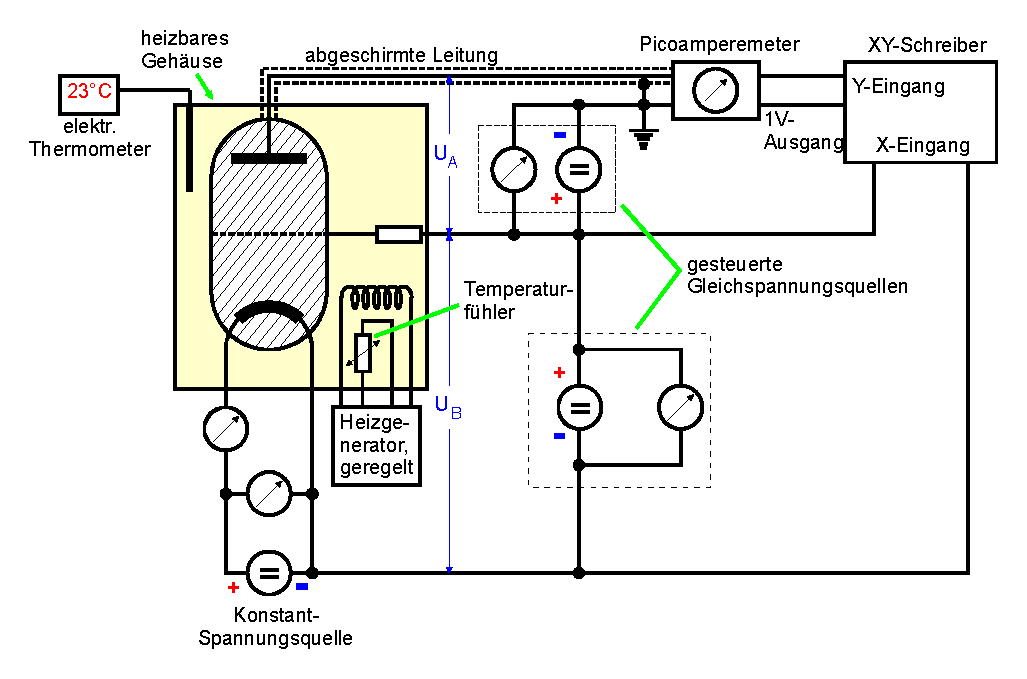
\includegraphics[width=0.8\linewidth]{pictures/schaltplan.pdf}
    \caption{Schaltung zur Aufnahme einer Franck-Hertz-Kurve \cite{v601}.}
    \label{fig:schaltung}
\end{figure}

In \autoref{fig:schaltung} is der Schaltplan zur Aufnahme der Franck-Hertz-Kurve dargestellt.
Die Umgebungstemperatur des Gefäßes wird mithilfe eines Heizgenerators gesteuert und mit einem Thermometer gemessen.
Mithilfe eines XY-Schreibers wird der Auffängerstrom, welcher mit einem Picoamperemeter an der Auffängerelektrode gemessen wird,
in Abhängigkeit der zu betrachtetem Spannung aufgezeichnet.
Dabei ist auf eine richtige Einstellung des Schreibers und auch des Picoamperemeters zu achten, damit die aufgenommene Kurve nicht den Zeichenbereich überschreitet.

Am Anfang der Messung wird bei einer Raumtemperatur von $T = \qty{25,2}{°C}$ der Auffängerstrom $I_\text{A}$ als Kurve in Abhängigkeit der Gegenspannung $U_\text{A}$ aufgezeichnet.
Dabei wird eine konstante Bremsspannung von $U_\text{B} = \qty{11}{\volt}$ eingestellt und $U_\text{A}$ von 0 bis $\qty{10}{\volt}$ variiert.
Dies wird für eine Temperatur von $T = \qty{160(1)}{°C}$ wiederholt. 
Danach werden weitere Stromkurven aufgenommen, welche jedoch in Abhängigkeit der Bremsspannung $U_\text{B}$ im Bereich von 0 bis $\qty{60}{\volt}$ ist.
Die erste wird für eine Temperatur von $T = \qty{175.4(1)}{°C}$ und die zweite von $T = \qty{185.9(3)}{°C}$ durchgeführt.
Bei allen Aufzeichnungen wird nach Schreiben der Kurve die Spannung in gleichmäßig gewählten Abständen zurückgeregelt und ein Punkt gesetzt.
